% ARPEGOS:  Automatized Roleplaying-game Profile Extensible Generator Ontology based System %
% Author : Alejandro Muñoz Del Álamo %
% Copyright 2019 %

% Section 2.2: Estado del Arte %

\section{Estado del Arte} \label{Estado_Arte}
Con el objetivo de simplificar el proceso de creación de personajes en los juegos de rol tradicionales, se han originado 
multitud de aplicaciones con diferentes funciones y finalidades. Algunas de las aplicaciones son referencias completas de 
los juegos, que sirven como elementos de consulta accesibles, rápidos y precisos. Un ejemplo de ello es 
\textit{\textbf{5e Character}}, mostrada en las figuras \ref*{5e_Character1} y \ref*{5e_Character2} que es una referencia 
completa de personajes para \textit{Dragones y Mazmorras, 5ª Edición}.\medskip

Estas aplicaciones ofrecen información del juego de manera accesible, pero no permiten aprovechar la 
digitalización de ésta para otros usos. Permiten realizar búsquedas rápidas, pero tampoco suelen disponer de 
toda la información del juego, de manera que para poder hacer consultas del juego completo es necesario 
acceder al libro del juego o hacer uso de más aplicaciones. Además, son aplicaciones que sólo pueden 
ser útiles para una versión específica del juego, ya que las versiones nuevas de los juegos de rol suelen 
incluir una gran cantidad de cambios. Aún así, éstas pueden no resultar obsoletas al momento de surgir la 
nueva versión, pues suele haber un período de transición entre versiones bastante amplio.
\newpage
% https://play.google.com/store/apps/details?id=com.dungeon.dev.a5echaracter&hl=en_US

\begin{figure}[H]
    \centering
    \begin{minipage}{0.38\textwidth}
        \centering
        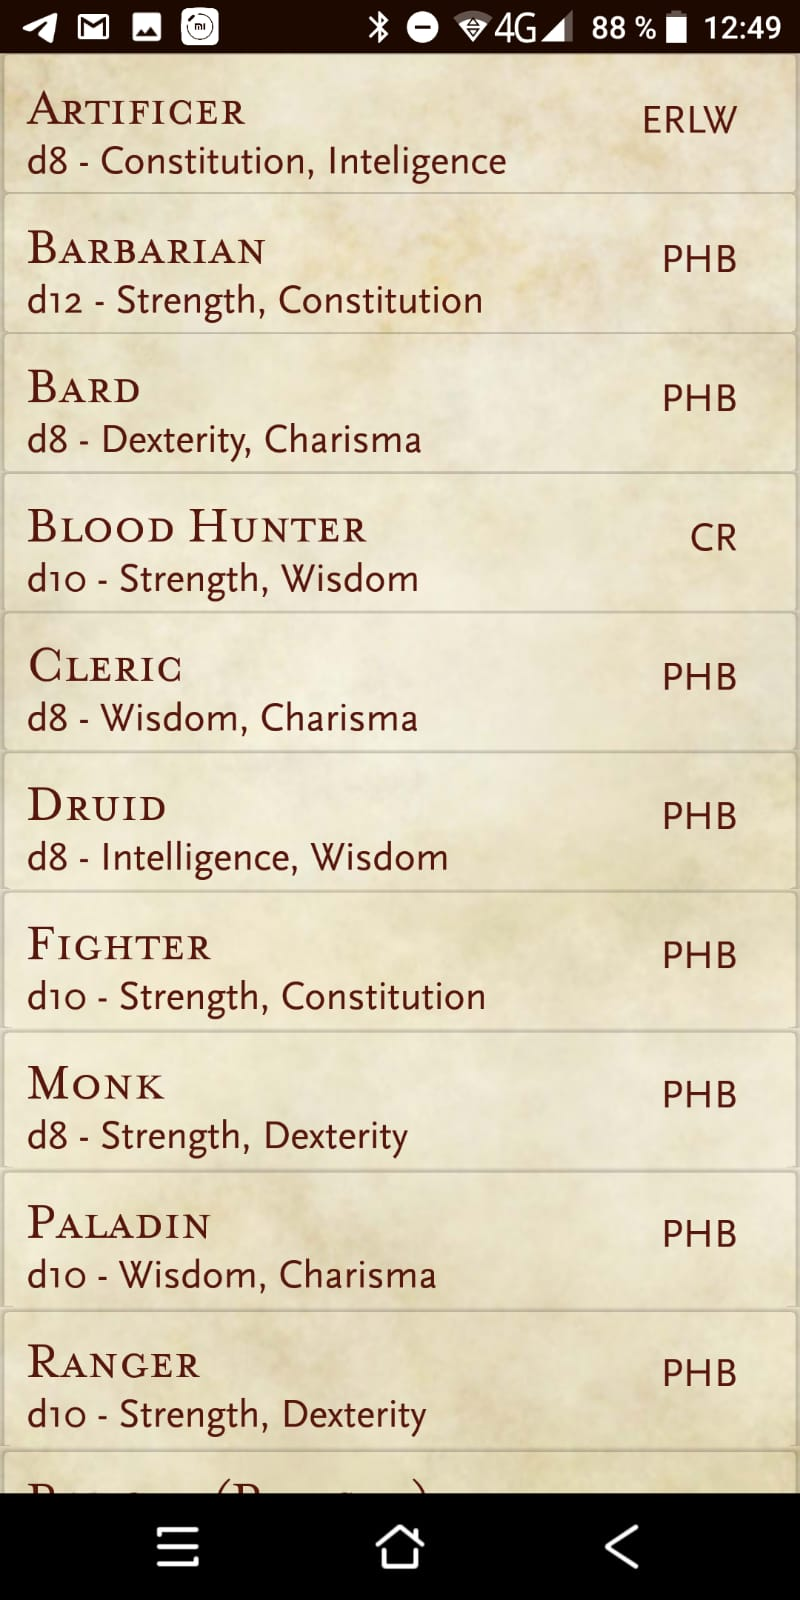
\includegraphics[width=0.5\textwidth]{Images/5e_Character_1.jpeg}
        \caption{\textit{\textbf{5e Character}}: Pantalla de selección 
        de clases}
        \label{5e_Character1}        
    \end{minipage} \hspace{2cm}
    \begin{minipage}{0.38\textwidth}
        \centering
        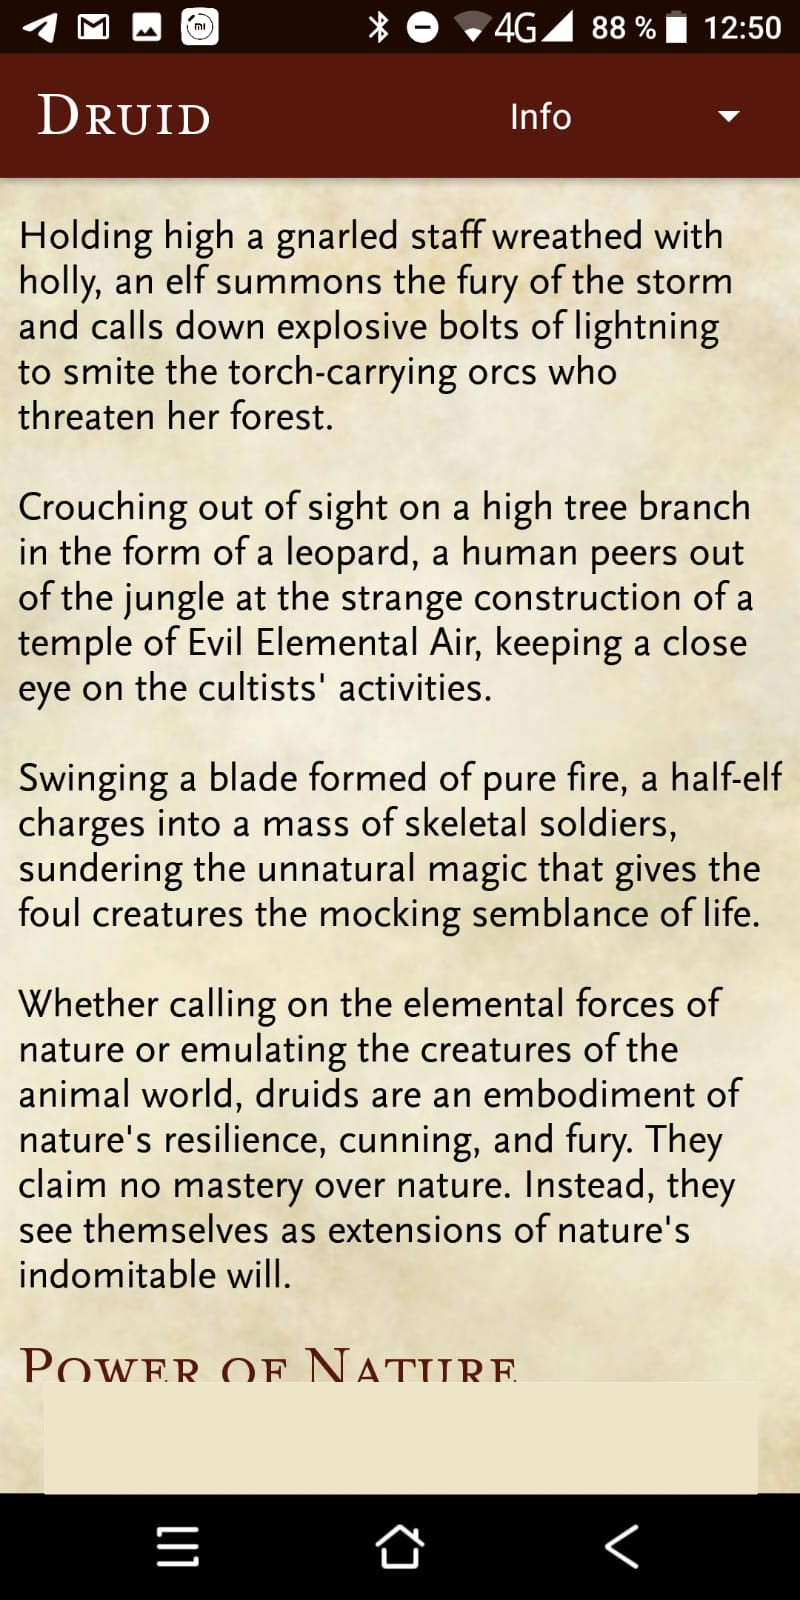
\includegraphics[width=0.5\textwidth]{Images/5e_Character_2.jpeg}
        \caption{\textit{\textbf{5e Character}}: Información 
        de la clase \textit{Druida}}
        \label{5e_Character2}        
    \end{minipage}
\end{figure}

Como en los juegos de rol se utilizan diferentes tipos de dados 
(de 3, 4, 6, 8, 10, 12, 20, 30 y hasta 100 lados), también podemos encontrar aplicaciones 
como \textit{\textbf{RPG Simple Dice}}, expuesta en las figuras \ref*{SimpleDice1} y \ref*{SimpleDice2} que están preparadas para simular los resultados 
de lanzar estos dados, lo cual hace que se conviertan en una herramienta útil si no 
disponemos de alguno de éstos.

\begin{figure}[H]
    \centering
    \begin{minipage}{0.35\textwidth}
        \centering
        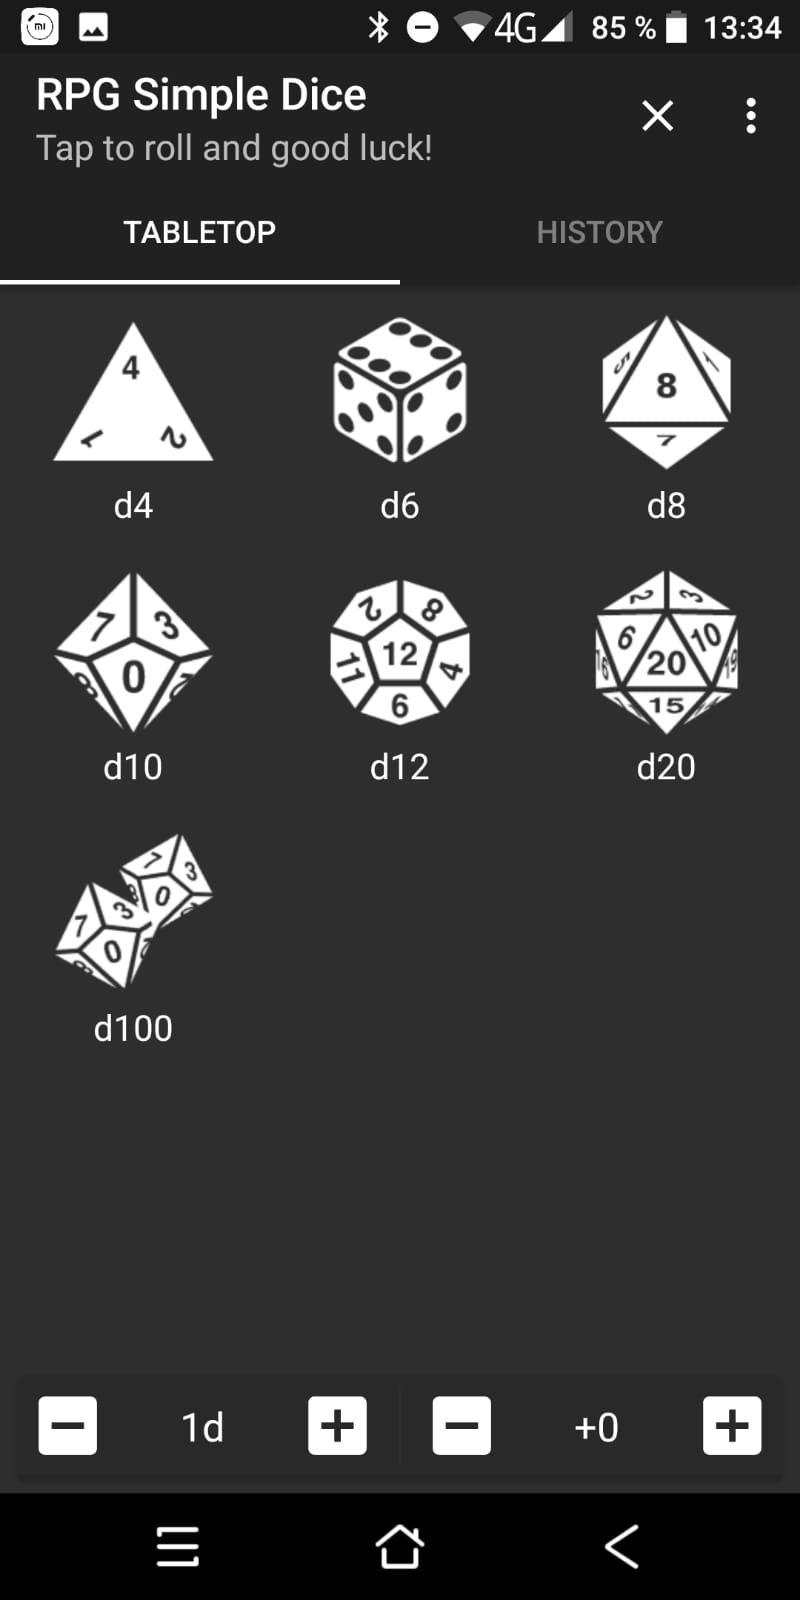
\includegraphics[width=0.5\textwidth]{Images/RPG_Simple_Dice_1.jpeg}
        \caption{\textit{\textbf{RPG Simple Dice}}: Pantalla de selección 
        de dados}
        \label{SimpleDice1}        
    \end{minipage} \hspace{2cm}
    \begin{minipage}{0.35\textwidth}
        \centering
        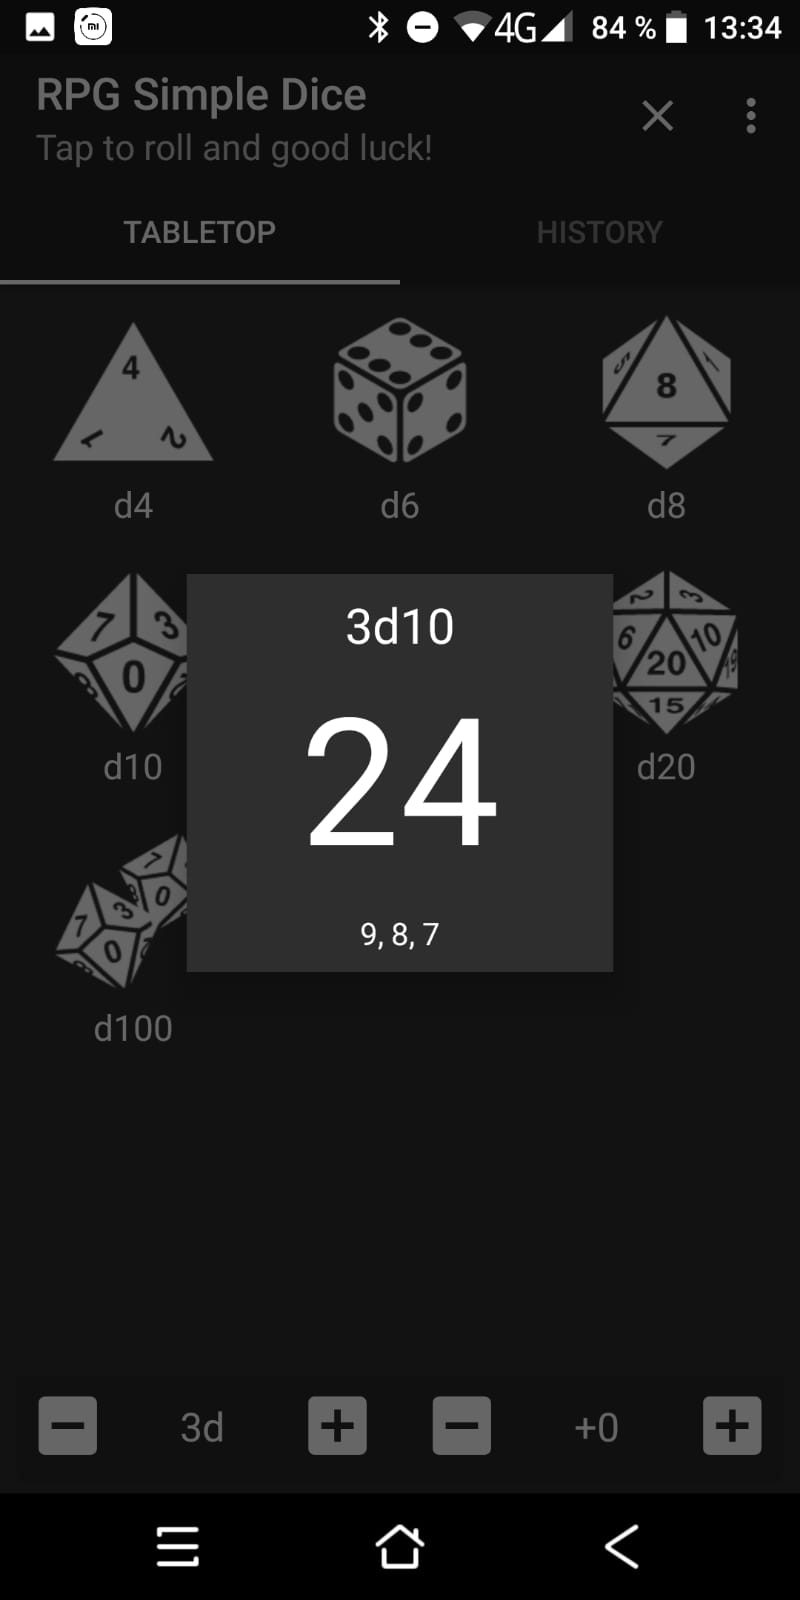
\includegraphics[width=0.5\textwidth]{Images/RPG_Simple_Dice_2.jpeg}
        \caption{\textit{\textbf{RPG Simple Dice}}: Ejemplo de lanzamiento de 
        dados}
        \label{SimpleDice2}        
    \end{minipage}
\end{figure}
\newpage
Otras aplicaciones proporcionan algunas herramientas que simplifican 
cálculos que resultan tediosos durante el transcurso de la partida, como 
es el caso de \textit{\textbf{BattleTrack}}, cuya interfaz se puede apreciar 
en las figuras \ref*{BattleTrack1} y \ref*{BattleTrack2}. Dependiendo de la aplicación 
que se utilice, puede incluir su propio simulador de dados, lo que hace 
innecesario el uso de aplicaciones específicas para ello. \medskip

El punto negativo de estas aplicaciones es que son generales y no disponen de 
la información específica de los personajes de los jugadores, de manera que 
el resultado es aproximado, o requiere que el usuario especifique previamente 
toda la información, lo que puede llegar a resultar tedioso si en una partida 
se realizan múltiples cálculos de éste tipo.


\begin{figure}[H]
    \centering
    \begin{minipage}{0.3\textwidth}
        \centering
        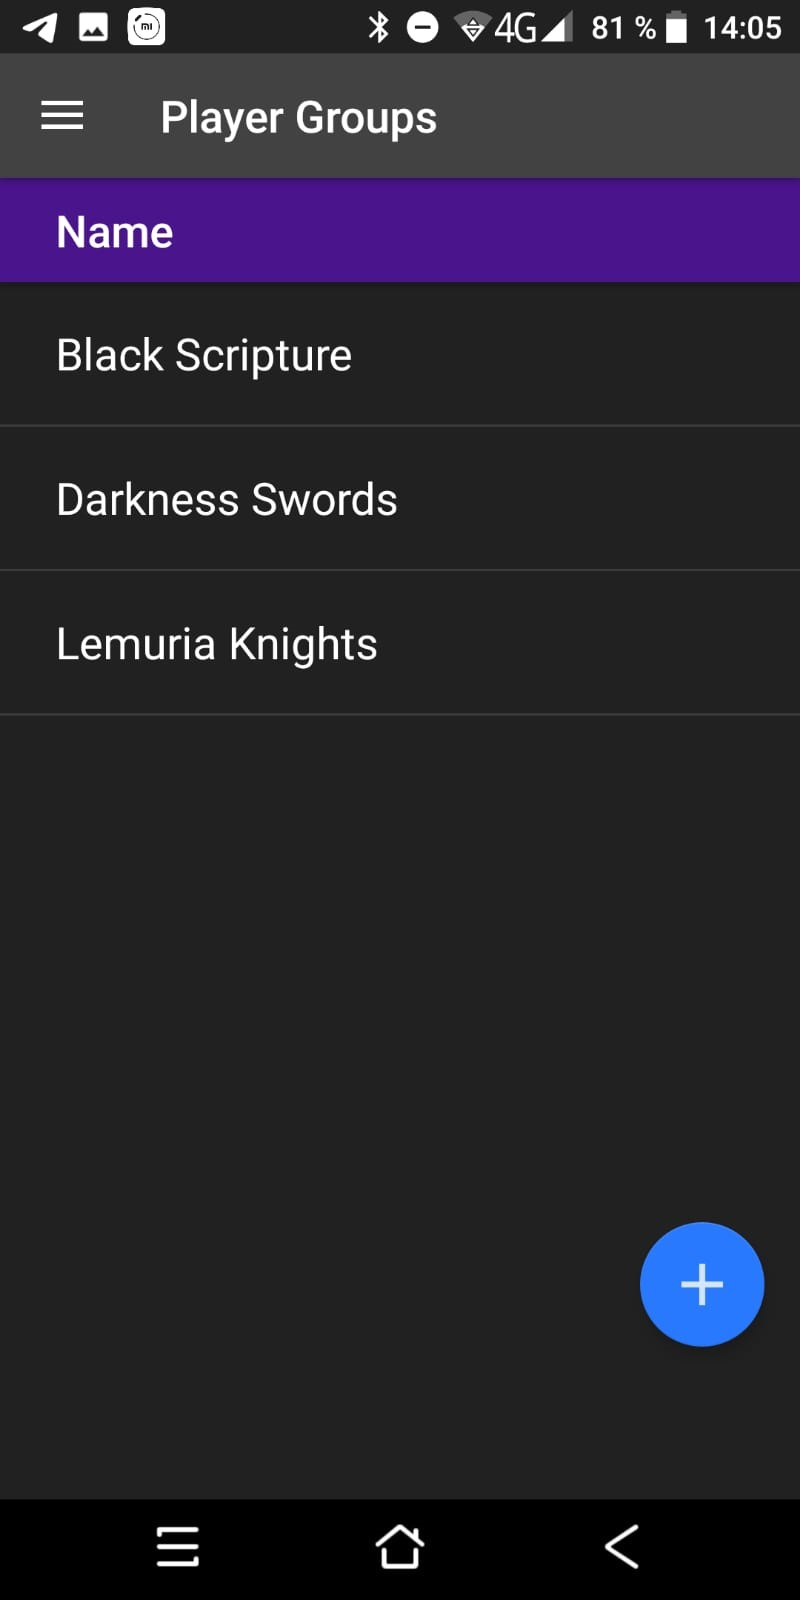
\includegraphics[width=0.7\textwidth]{Images/BattleTrack_1.jpeg}
        \caption{\textit{\textbf{BattleTrack}}: Pantalla de grupos }
        \label{BattleTrack1}   
        
    \end{minipage} \hspace{2cm}
    \begin{minipage}{0.3\textwidth}
        \centering
        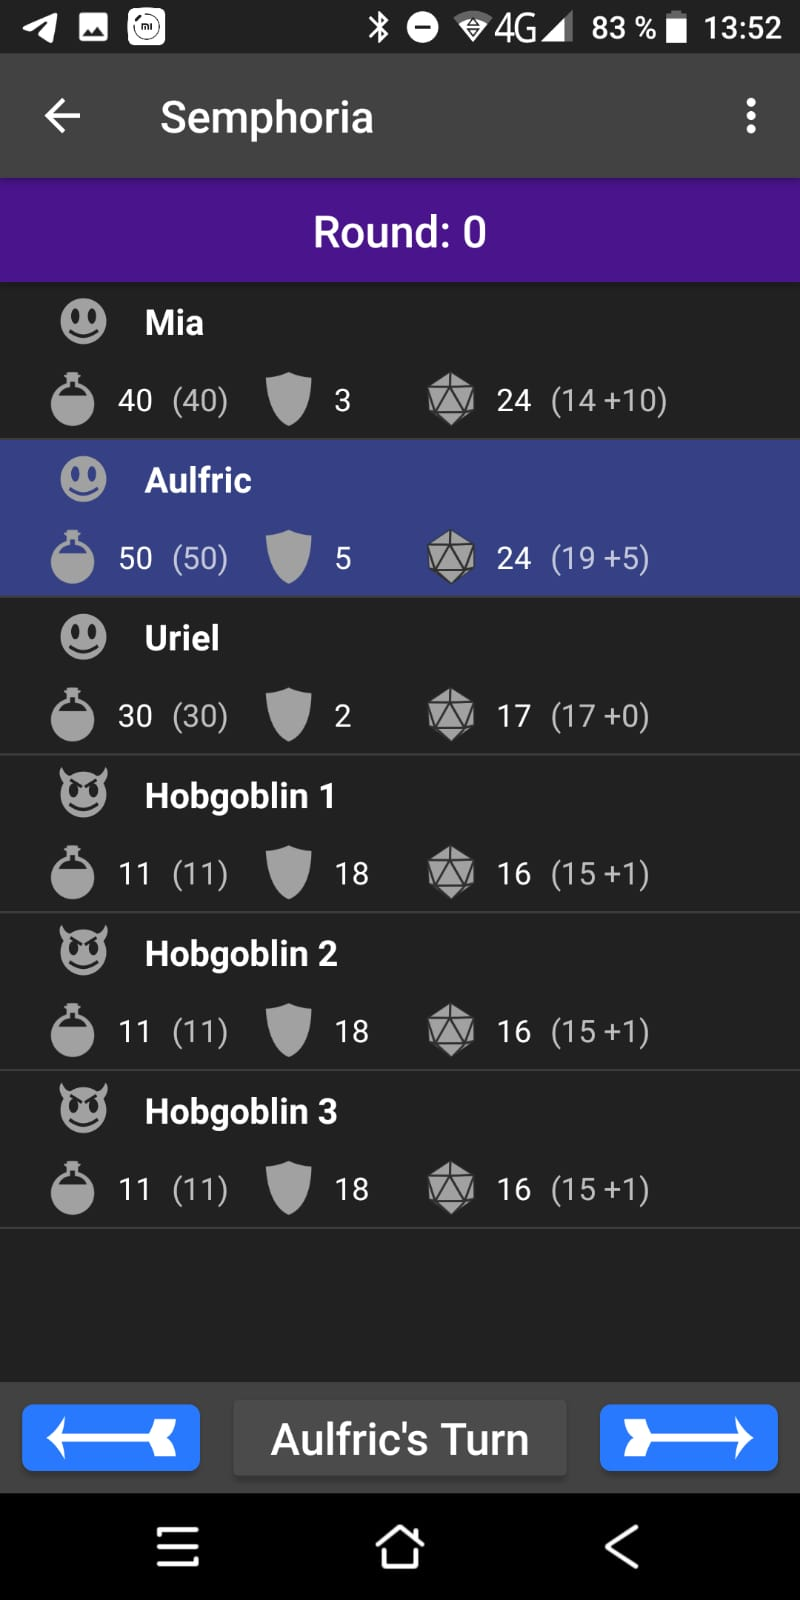
\includegraphics[width=0.7\textwidth]{Images/BattleTrack_2.jpeg}
        \caption{\textit{\textbf{BattleTrack}}: Ejemplo de combate}
        \label{BattleTrack2}           
    \end{minipage}
\end{figure}
Con el fin de ayudar en la ambientación, aplicaciones como 
\textit{\textbf{RPGSound}} (Figuras \ref*{RPGSound1} y \ref*{RPGSound2}) 
aportan bibliotecas de sonido que se pueden 
utilizar durante la representación de la partida para sumirse en ella.
\newpage
\begin{figure}[H]
    \centering
    \begin{minipage}{0.3\textwidth}
        \centering
        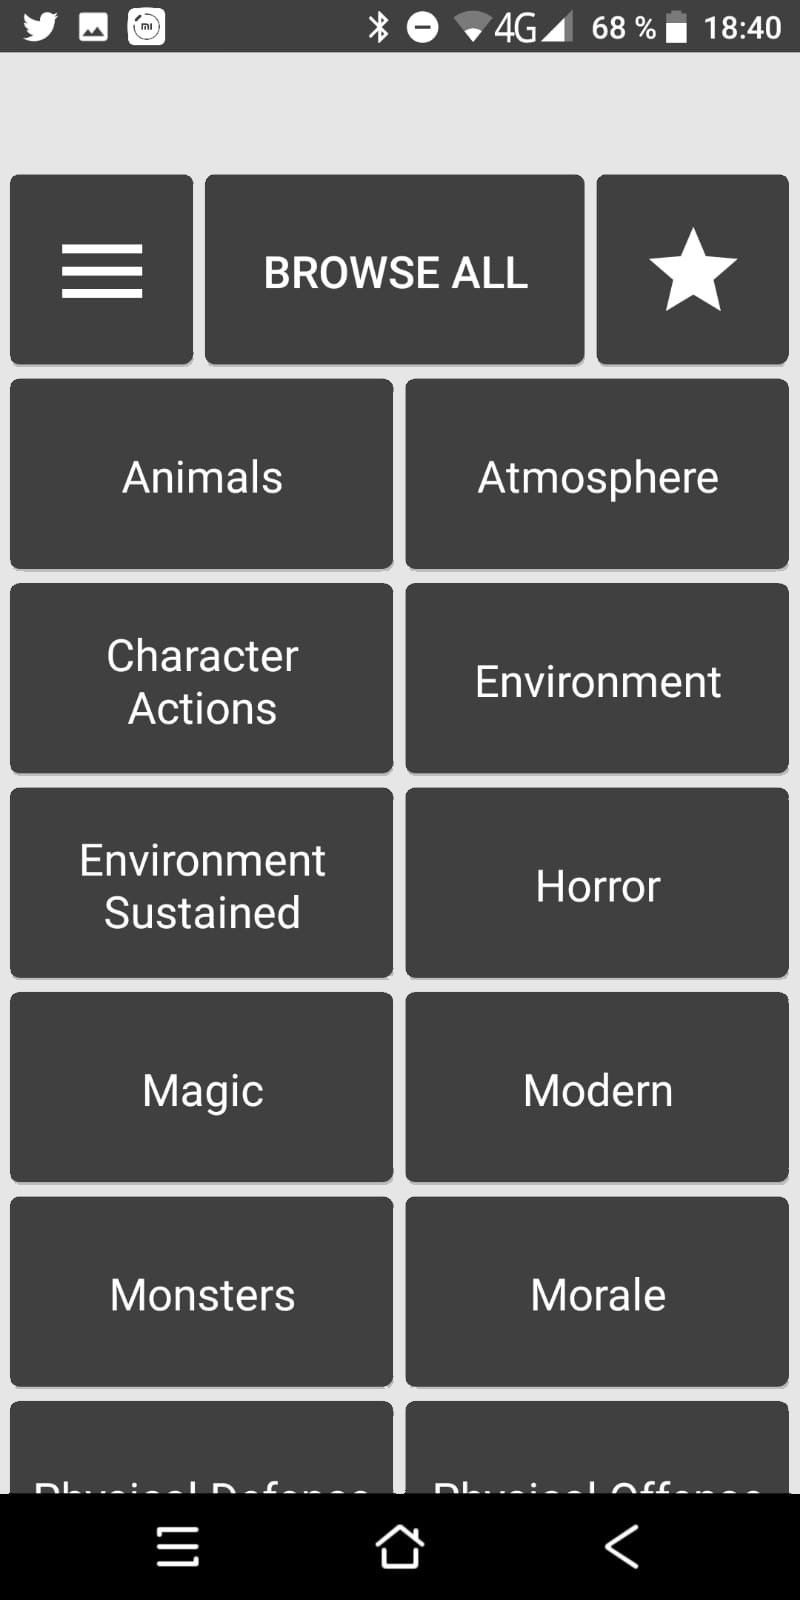
\includegraphics[width=0.7\textwidth]{Images/RPGSound_1.jpeg}
        \caption{\textit{\textbf{RPGSound}}: Menú principal}
        \label{RPGSound1} 
    \end{minipage} \hspace{2cm}
    \begin{minipage}{0.3\textwidth}
        \centering
        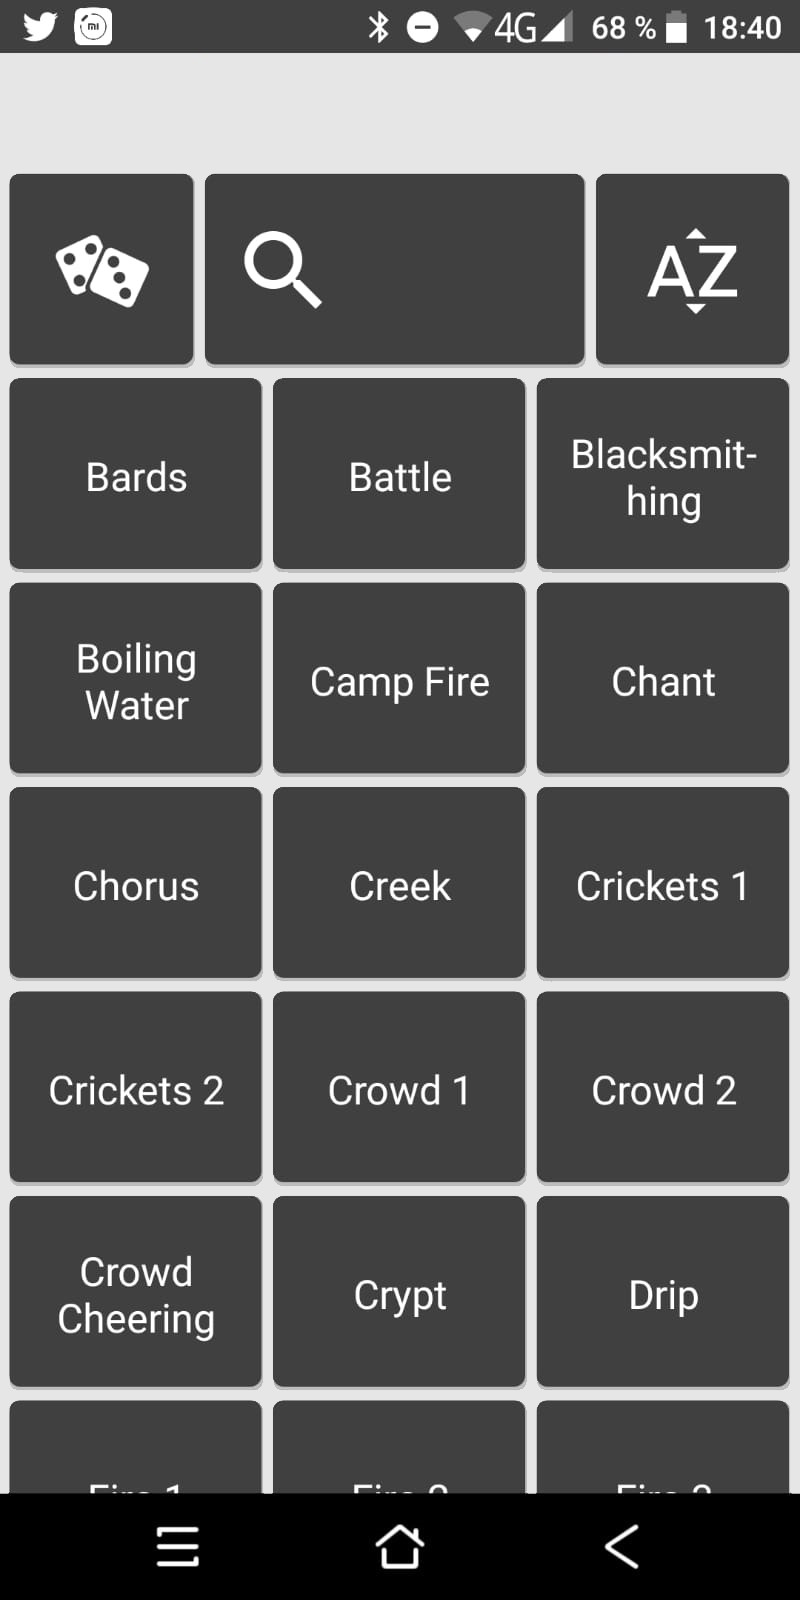
\includegraphics[width=0.7\textwidth]{Images/RPGSound_2.jpeg}
        \caption{\textit{\textbf{RPGSound}}: Menú de \textit{Ambiente}}
        \label{RPGSound2} 
    \end{minipage}
\end{figure}

Finalmente, quedan las aplicaciones conocidas como \textit{generadores de
personaje}, que permiten al usuario crear personajes para formar parte de 
una partida de rol, y acceder a esa información de forma rápida. Un buen 
ejemplo de esto es \textit{\textbf{RPG Character Sheet}}, como se muestra en 
las figuras \ref*{RPGCharacterSheet1} y \ref*{RPGCharacterSheet2}. 
\begin{figure}[H]
    \centering
    \begin{minipage}{0.3\textwidth}
        \centering
        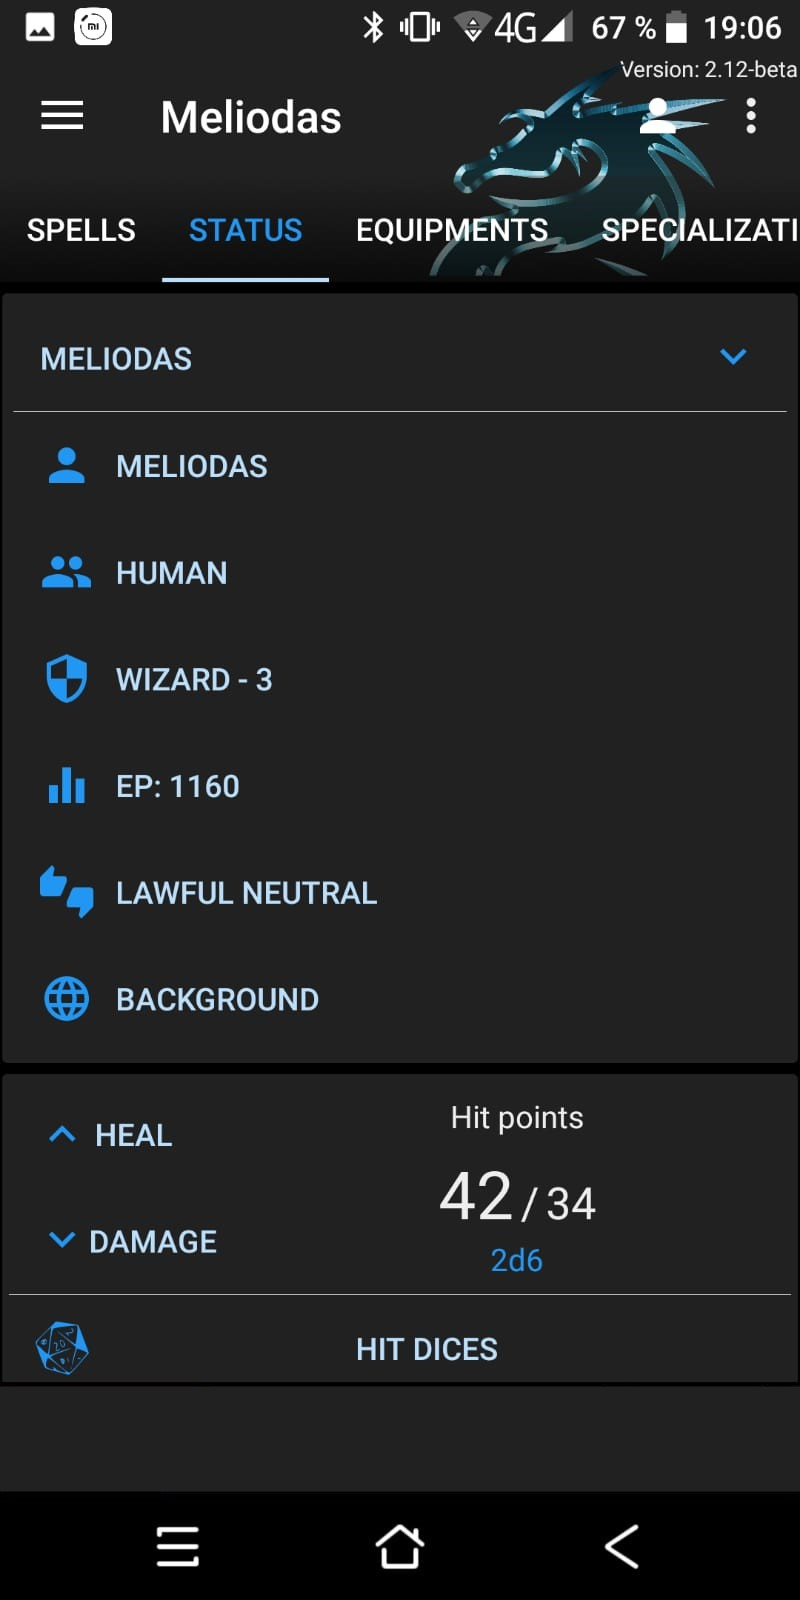
\includegraphics[width=0.7\textwidth]{Images/RPG_Character_Sheet_1.jpeg}
        \caption{\textit{\textbf{RPG Character Sheet}}: Pantalla de \textit{Estado}}
        \label{RPGCharacterSheet1}
    \end{minipage} \hspace{2cm}
    \begin{minipage}{0.3\textwidth}
        \centering
        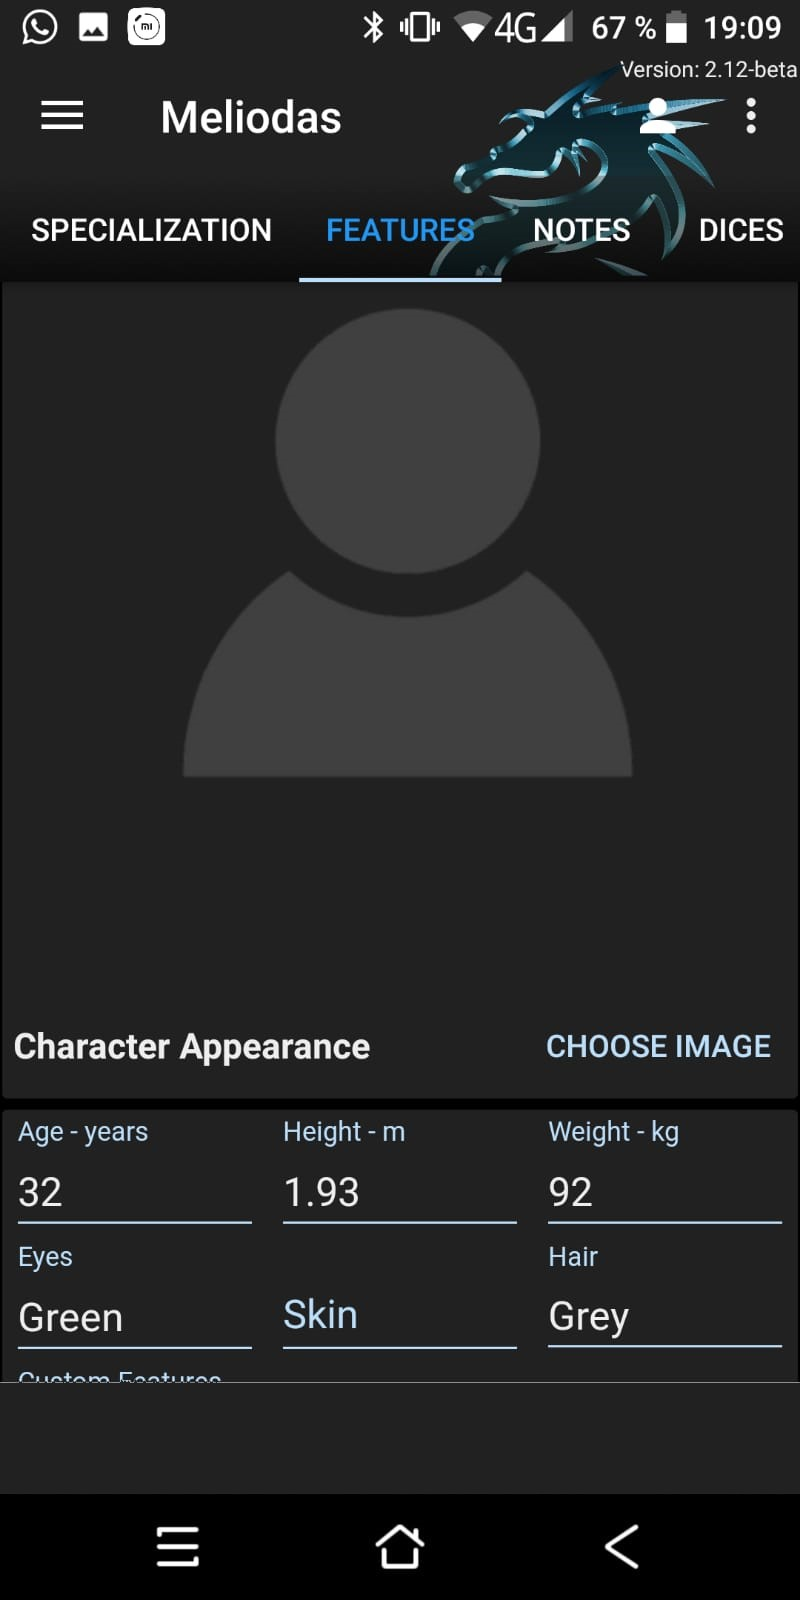
\includegraphics[width=0.7\textwidth]{Images/RPG_Character_Sheet_2.jpeg}
        \caption{\textit{\textbf{RPG Character Sheet}}: Pantalla de \textit{Features}}
        \label{RPGCharacterSheet2}
    \end{minipage}
\end{figure}
Aunque estas aplicaciones 
suelen reunir las funcionalidades de la mayoría de las aplicaciones previamente 
explicadas, suelen tener una interfaz bastante caótica, lo que resulta en una 
curva de aprendizaje bastante elevada para usuarios nuevos, que acaban 
prefiriendo el método tradicional, o el uso de varias aplicaciones más sencillas.

En resumen, hay un amplio abanico de aplicaciones que buscan resultar de utilidad a los 
jugadores de \textit{RPG} de diferentes maneras, ya sea facilitando la búsqueda de información, 
realizando los cálculos de los valores finales de las tiradas de dados o generando la información
de los personajes que forman parte de la partida.